\section{The {\large\textbf{\sys}} Architecture}

\begin{figure}[h]
    \centering
        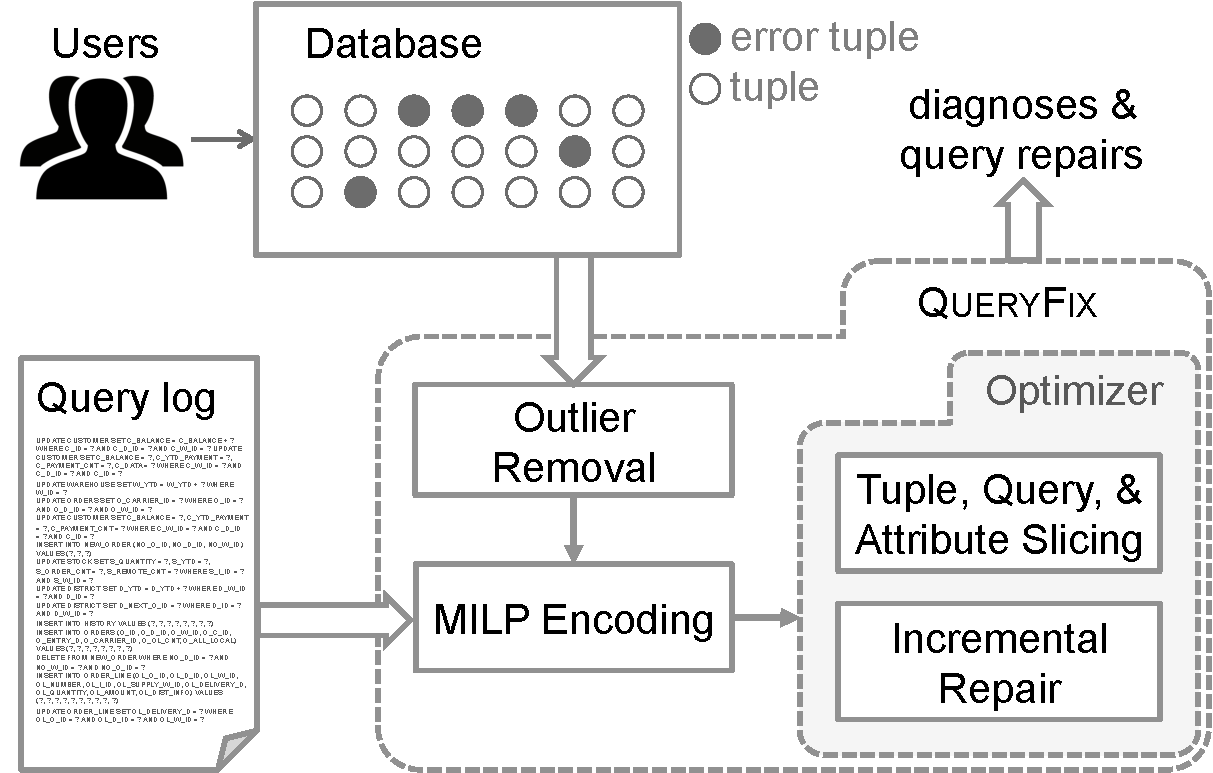
\includegraphics[scale=0.3]{figures/architecture}
    %\caption{\sys processes data anomalies in the form of complaints and analyzes logged query histories to identify the causes of error. 
    %In the heart of the system, the diagnosis problem is translated into a mixed integer linear program, and optimization modules ensure that the MILP programs can be evaluated efficiently.}
    \caption{\sys architecture diagram}
    \label{fig:architecture}
    \vspace*{-0.1in}
\end{figure}


Figure~\ref{fig:architecture} shows \sys's major components.  \sys takes as input 
a query log containing UPDATE, INSERT and DELETE queries, the database, along with a
set of identified data errors (called {\it complaints}).  These complaints are pairs
of tuple id of tuples that are wrong, along with an estimate of their correct values 
(e.g., $21500$ as tuple $t_3$'s tax value in Example~\ref{ex:telco}).
\sys uses this information to trace the causes of the errors and output the most likely set of 
queries in the log ({\it diagnoses}), along with proposed {\it repairs} of these queries.

To achieve this, \sys first performs an optional outlier removal step to deal with potential
false positives in the complaints.  Then the {\it MILP Encoding} component transforms the
query diagnosis problem into a Mixed Integer Linear Program (MILP) that is further optimized
through slicing and incremental repair techniques, before being sent
to an industrial MILP solver.  The output of the solver constitutes solutions to the query diagnosis
problem.
